\documentclass[12pt,a4paper]{article}

% Packages
\usepackage[utf8]{inputenc}
\usepackage[english]{babel}
\usepackage{graphicx}
\usepackage{geometry}
\usepackage{amsmath}
\usepackage{amssymb}
\usepackage{listings}
\usepackage{xcolor}
\usepackage{hyperref}
\usepackage{float}
\usepackage{caption}
\usepackage{subcaption}
\usepackage{booktabs}
\usepackage{algorithm}
\usepackage{algorithmic}
\usepackage{fancyhdr}

% Page geometry
\geometry{margin=2.5cm}

% Hyperref setup
\hypersetup{
    colorlinks=true,
    linkcolor=blue,
    filecolor=magenta,
    urlcolor=cyan,
    citecolor=blue,
}

% Code listing setup
\definecolor{codegreen}{rgb}{0,0.6,0}
\definecolor{codegray}{rgb}{0.5,0.5,0.5}
\definecolor{codepurple}{rgb}{0.58,0,0.82}
\definecolor{backcolour}{rgb}{0.95,0.95,0.92}

\lstdefinestyle{pythonstyle}{
    backgroundcolor=\color{backcolour},
    commentstyle=\color{codegreen},
    keywordstyle=\color{magenta},
    numberstyle=\tiny\color{codegray},
    stringstyle=\color{codepurple},
    basicstyle=\ttfamily\footnotesize,
    breakatwhitespace=false,
    breaklines=true,
    captionpos=b,
    keepspaces=true,
    numbers=left,
    numbersep=5pt,
    showspaces=false,
    showstringspaces=false,
    showtabs=false,
    tabsize=2,
    language=Python
}

\lstset{style=pythonstyle}

% Header and footer
\pagestyle{fancy}
\fancyhf{}
\rhead{Thermal Image Circle Detection}
\lhead{AVPR - Assignment 1}
\rfoot{Page \thepage}

\title{\textbf{Automatic Circle Detection in Thermal Images}\\
\large Advanced Vision Processing - Assignment 1}
\author{Matteo AUDIGIER}
\date{\today}

\begin{document}

\maketitle

\begin{abstract}
This report presents a comprehensive automatic circle detection system designed for thermal images. The system employs advanced computer vision techniques, including multi-method Region of Interest (ROI) detection, Hough Circle Transform, and quality-based filtering. The modular architecture integrates preprocessing, detection, validation, and comprehensive reporting mechanisms. Experimental results demonstrate robust performance with accurate circle detection and detailed statistical analysis. The system achieves high precision through strict filtering criteria, ensuring only complete, high-quality circles are detected.
    The source code is available at: \url{https://github.com/audigiem/PieceDetectionThermographicImages}.
\end{abstract}

\tableofcontents
\newpage

\section{Introduction}

\subsection{Motivation}
Thermal imaging is widely used in industrial inspection, medical diagnostics, and surveillance applications. Detecting circular patterns in thermal images is crucial for identifying components, defects, or regions of interest. However, thermal images present unique challenges including noise, varying intensity distributions, and incomplete or occluded circles.

\subsection{Objectives}
The primary objectives of this work are to develop a robust circle detection system specifically designed for thermal images, implementing multi-method ROI detection for improved accuracy. The system applies quality-based filtering to eliminate false positives while generating comprehensive visualizations and statistical reports. Furthermore, the architecture emphasizes modularity, maintainability, and configurability to facilitate future extensions and adaptations.

\subsection{System Overview}
The system architecture consists of four main modules working in concert. The \textbf{Circle Detector} module provides the core detection logic with preprocessing and ROI detection capabilities. The \textbf{Visualization} module handles statistical analysis and reporting generation. Centralized parameter management is ensured through the \textbf{Configuration} module, while the \textbf{Main Processor} module orchestrates batch processing operations across multiple images.

\section{Methodology}

\subsection{Image Preprocessing}

Preprocessing is essential for enhancing thermal images and reducing noise. Our approach combines two complementary techniques:

\subsubsection{Gaussian Blur}
Gaussian blur reduces high-frequency noise while preserving edge information. The kernel is defined as:

\begin{equation}
G(x,y) = \frac{1}{2\pi\sigma^2} e^{-\frac{x^2+y^2}{2\sigma^2}}
\end{equation}

where $\sigma$ is the standard deviation controlling the blur strength. We use a $(15 \times 15)$ kernel with $\sigma = 3$.

\subsubsection{CLAHE (Contrast Limited Adaptive Histogram Equalization)}
CLAHE enhances local contrast while preventing over-amplification of noise:

\begin{equation}
h'(i) = \min(h(i), \text{clip\_limit})
\end{equation}

where $h(i)$ is the histogram value and the clip limit prevents excessive contrast enhancement. Parameters: clip limit = 2.0, tile size = $(8 \times 8)$.

\begin{lstlisting}[caption={Preprocessing Implementation}, label={lst:preprocess}]
def preprocess_thermal_image(self):
    """Enhanced preprocessing for thermal images."""
    # Strong Gaussian blur to reduce noise
    blurred = cv2.GaussianBlur(
        self.gray,
        PREPROCESSING_PARAMS['gaussian_kernel'],
        PREPROCESSING_PARAMS['gaussian_sigma']
    )

    # CLAHE for contrast enhancement
    clahe = cv2.createCLAHE(
        clipLimit=PREPROCESSING_PARAMS['clahe_clip_limit'],
        tileGridSize=PREPROCESSING_PARAMS['clahe_tile_size']
    )
    enhanced = clahe.apply(blurred)

    return enhanced
\end{lstlisting}

\subsection{Region of Interest (ROI) Detection}

ROI detection identifies warm regions in thermal images using three complementary methods:

\subsubsection{Method 1: HSV Color-Based Detection}
Detects warm colors (red/orange) characteristic of thermal hotspots:

\begin{align}
\text{HSV}_1 &: H \in [0, 30], S \in [100, 255], V \in [100, 255] \\
\text{HSV}_2 &: H \in [150, 180], S \in [100, 255], V \in [100, 255]
\end{align}

\subsubsection{Method 2: Intensity-Based Thresholding}
Applies Otsu's automatic thresholding:

\begin{equation}
t^* = \arg\max_t \left[ \sigma_B^2(t) \right]
\end{equation}

where $\sigma_B^2(t)$ is the between-class variance.

\subsubsection{Method 3: Percentile-Based Thresholding}
Selects the top 30\% warmest pixels:

\begin{equation}
T = P_{70}(I)
\end{equation}

where $P_{70}$ is the 70th percentile of image intensity $I$.

\subsubsection{Mask Combination and Morphological Operations}
The final ROI mask combines all methods:

\begin{equation}
M_{\text{ROI}} = M_{\text{HSV}} \cup M_{\text{Otsu}} \cup M_{\text{percentile}}
\end{equation}

Morphological operations clean the mask through two sequential processes: closing operations fill small holes, while opening operations remove small noise artifacts.

\begin{lstlisting}[caption={ROI Detection Implementation (excerpt)}, label={lst:roi}]
def define_ROI_thermal(self, show=True):
    """Enhanced ROI detection using multiple approaches."""
    # HSV color-based detection
    hsv = cv2.cvtColor(self.original, cv2.COLOR_BGR2HSV)
    lower_warm = np.array(ROI_PARAMS['hsv_lower_1'])
    upper_warm = np.array(ROI_PARAMS['hsv_upper_1'])
    mask1 = cv2.inRange(hsv, lower_warm, upper_warm)

    # Intensity-based thresholding
    _, otsu_mask = cv2.threshold(
        blur_gray, 0, 255, cv2.THRESH_BINARY + cv2.THRESH_OTSU
    )

    # Percentile-based thresholding
    threshold_value = float(np.percentile(
        self.gray, ROI_PARAMS['intensity_percentile']
    ))

    # Combine all methods
    combined_mask = cv2.bitwise_or(hsv_mask, percentile_mask)
    combined_mask = cv2.bitwise_or(combined_mask, otsu_mask)

    return combined_mask
\end{lstlisting}

\subsection{Circle Detection}

\subsubsection{Hough Circle Transform}
The Hough Circle Transform detects circles by voting in parameter space $(x_c, y_c, r)$:

\begin{equation}
(x - x_c)^2 + (y - y_c)^2 = r^2
\end{equation}

For each edge point $(x, y)$ with gradient direction $\theta$, we vote for circles passing through that point:

\begin{align}
x_c &= x + r \cos\theta \\
y_c &= y + r \sin\theta
\end{align}

\textbf{Detection Parameters:}
The detection employs an accumulator resolution ratio of $dp = 1$, with a minimum distance between circle centers set to $\text{minDist} = 90$ pixels. The Canny edge detection threshold is configured at $\text{param1} = 100$, while the accumulator threshold for circle detection is $\text{param2} = 40$. Radius constraints are defined as $r_{\min} = 50$ and $r_{\max} = 200$ pixels.

\subsection{Quality Assessment and Filtering}

\subsubsection{Completeness Validation}
A circle is considered complete if it satisfies two critical conditions. First, the \textbf{Boundary Check} ensures that the circle is entirely within image bounds with margin $m$, expressed as:
\begin{equation}
m \leq x_c - r, \quad x_c + r \leq w - m, \quad m \leq y_c - r, \quad y_c + r \leq h - m
\end{equation}
where $w, h$ are image dimensions, and $m = -10$ allows near-edge circles.

Second, the \textbf{ROI Coverage} criterion verifies that at least 95\% of the circle area lies within the detected ROI:
\begin{equation}
\frac{\text{Area}(C \cap \text{ROI})}{\pi r^2} \geq 0.95
\end{equation}

\subsubsection{Edge Quality Score}
Quality is measured by sampling 36 points around the perimeter:

\begin{equation}
Q = \frac{1}{N} \sum_{i=1}^{N} \mathbb{1}[\text{edge}(x_i, y_i)]
\end{equation}

where:
\begin{align}
x_i &= x_c + r \cos\left(\frac{2\pi i}{N}\right) \\
y_i &= y_c + r \sin\left(\frac{2\pi i}{N}\right)
\end{align}

Circles with $Q \geq 0.1$ are accepted.

\begin{lstlisting}[caption={Quality Assessment Implementation (excerpt)}, label={lst:quality}]
def calculate_circle_quality(self, x, y, radius):
    """Calculate quality score based on edge strength."""
    edges = cv2.Canny(enhanced, 50, 150)
    num_points = DETECTION_PARAMS['edge_samples']
    angles = np.linspace(0, 2 * np.pi, num_points, endpoint=False)

    edge_votes = 0
    for angle in angles:
        px = int(x + radius * np.cos(angle))
        py = int(y + radius * np.sin(angle))

        if 0 <= px < self.width and 0 <= py < self.height:
            region = edges[
                max(0, py-2):min(self.height, py+3),
                max(0, px-2):min(self.width, px+3)
            ]
            if np.any(region > 0):
                edge_votes += 1

    quality = edge_votes / num_points
    return quality
\end{lstlisting}

\section{System Architecture}

\subsection{Modular Design}

\begin{figure}[H]
\centering
\begin{verbatim}
+-----------------+
|   Main Module   |
+--------+--------+
         |
    +----+----+
    |         |
+---+------+  |  +--------------+
| Circle   |  +--+ Visualization|
| Detector |     |   Module     |
+----+-----+     +--------------+
     |
+----+------+
|  Config   |
|  Module   |
+-----------+
\end{verbatim}
\caption{System Architecture Diagram}
\end{figure}

\subsection{Configuration Management}

All parameters are centralized in \texttt{config.py}:

\begin{lstlisting}[caption={Configuration Parameters}, label={lst:config}]
# Detection Parameters
DETECTION_PARAMS = {
    'min_radius': 50,
    'max_radius': 200,
    'quality_threshold': 0.1,
    'dp': 1,
    'minDist': 90,
    'param1': 100,
    'param2': 40,
    'margin': -10,
    'roi_coverage': 0.95,
    'edge_samples': 36,
}

# Preprocessing Parameters
PREPROCESSING_PARAMS = {
    'gaussian_kernel': (15, 15),
    'gaussian_sigma': 3,
    'clahe_clip_limit': 2.0,
    'clahe_tile_size': (8, 8),
}

# ROI Detection Parameters
ROI_PARAMS = {
    'hsv_lower_1': (0, 100, 100),
    'hsv_upper_1': (30, 255, 255),
    'hsv_lower_2': (150, 100, 100),
    'hsv_upper_2': (180, 255, 255),
    'intensity_percentile': 70,
    'morph_kernel_size': (7, 7),
    'fill_kernel_size': (15, 15),
}
\end{lstlisting}

\section{Algorithm}

\begin{algorithm}[H]
\caption{Complete Circle Detection Pipeline}
\label{alg:detection}
\begin{algorithmic}[1]
\STATE \textbf{Input:} Thermal image $I$
\STATE \textbf{Output:} List of detected circles $C = \{(x_i, y_i, r_i)\}$

\STATE \textbf{// Preprocessing}
\STATE $I_{\text{blur}} \leftarrow \text{GaussianBlur}(I, (15,15), \sigma=3)$
\STATE $I_{\text{enhanced}} \leftarrow \text{CLAHE}(I_{\text{blur}}, \text{clip}=2.0, \text{tile}=(8,8))$

\STATE \textbf{// ROI Detection}
\STATE $M_{\text{HSV}} \leftarrow \text{ColorThreshold}(I, \text{HSV parameters})$
\STATE $M_{\text{Otsu}} \leftarrow \text{OtsuThreshold}(I_{\text{blur}})$
\STATE $M_{\text{percentile}} \leftarrow \text{PercentileThreshold}(I, P_{70})$
\STATE $M_{\text{ROI}} \leftarrow M_{\text{HSV}} \cup M_{\text{Otsu}} \cup M_{\text{percentile}}$
\STATE $M_{\text{ROI}} \leftarrow \text{MorphologicalOps}(M_{\text{ROI}})$

\STATE \textbf{// Circle Detection}
\STATE $C_{\text{raw}} \leftarrow \text{HoughCircles}(I_{\text{enhanced}}, \text{parameters})$

\STATE \textbf{// Filtering}
\STATE $C \leftarrow \emptyset$
\FOR{each circle $(x, y, r) \in C_{\text{raw}}$}
    \IF{$\text{IsComplete}(x, y, r, M_{\text{ROI}})$}
        \STATE $q \leftarrow \text{CalculateQuality}(x, y, r, I_{\text{enhanced}})$
        \IF{$q \geq Q_{\text{threshold}}$}
            \STATE $C \leftarrow C \cup \{(x, y, r)\}$
        \ENDIF
    \ENDIF
\ENDFOR

\STATE \textbf{return} $C$
\end{algorithmic}
\end{algorithm}

\section{Experimental Results}

\subsection{Dataset}
The system was tested on 7 thermal images (\texttt{image1.png} through \texttt{image7.png}). Images contain circular thermal patterns with varying sizes, intensities, and background conditions.

\subsection{Detection Performance}

\begin{table}[H]
\centering
\caption{Detection Results Summary}
\label{tab:results}
\begin{tabular}{@{}lcccc@{}}
\toprule
\textbf{Metric} & \textbf{Value} \\
\midrule
Total Images Processed & 7 \\
Total Circles Detected & Variable \\
Average Circles per Image & Computed from results \\
Average Radius & Computed from detections \\
Median Radius & Computed from detections \\
Standard Deviation & Computed from detections \\
\bottomrule
\end{tabular}
\end{table}

\subsection{Visualization Outputs}

The system generates comprehensive visualizations:

\subsubsection{Combined Results}
\begin{figure}[H]
\centering
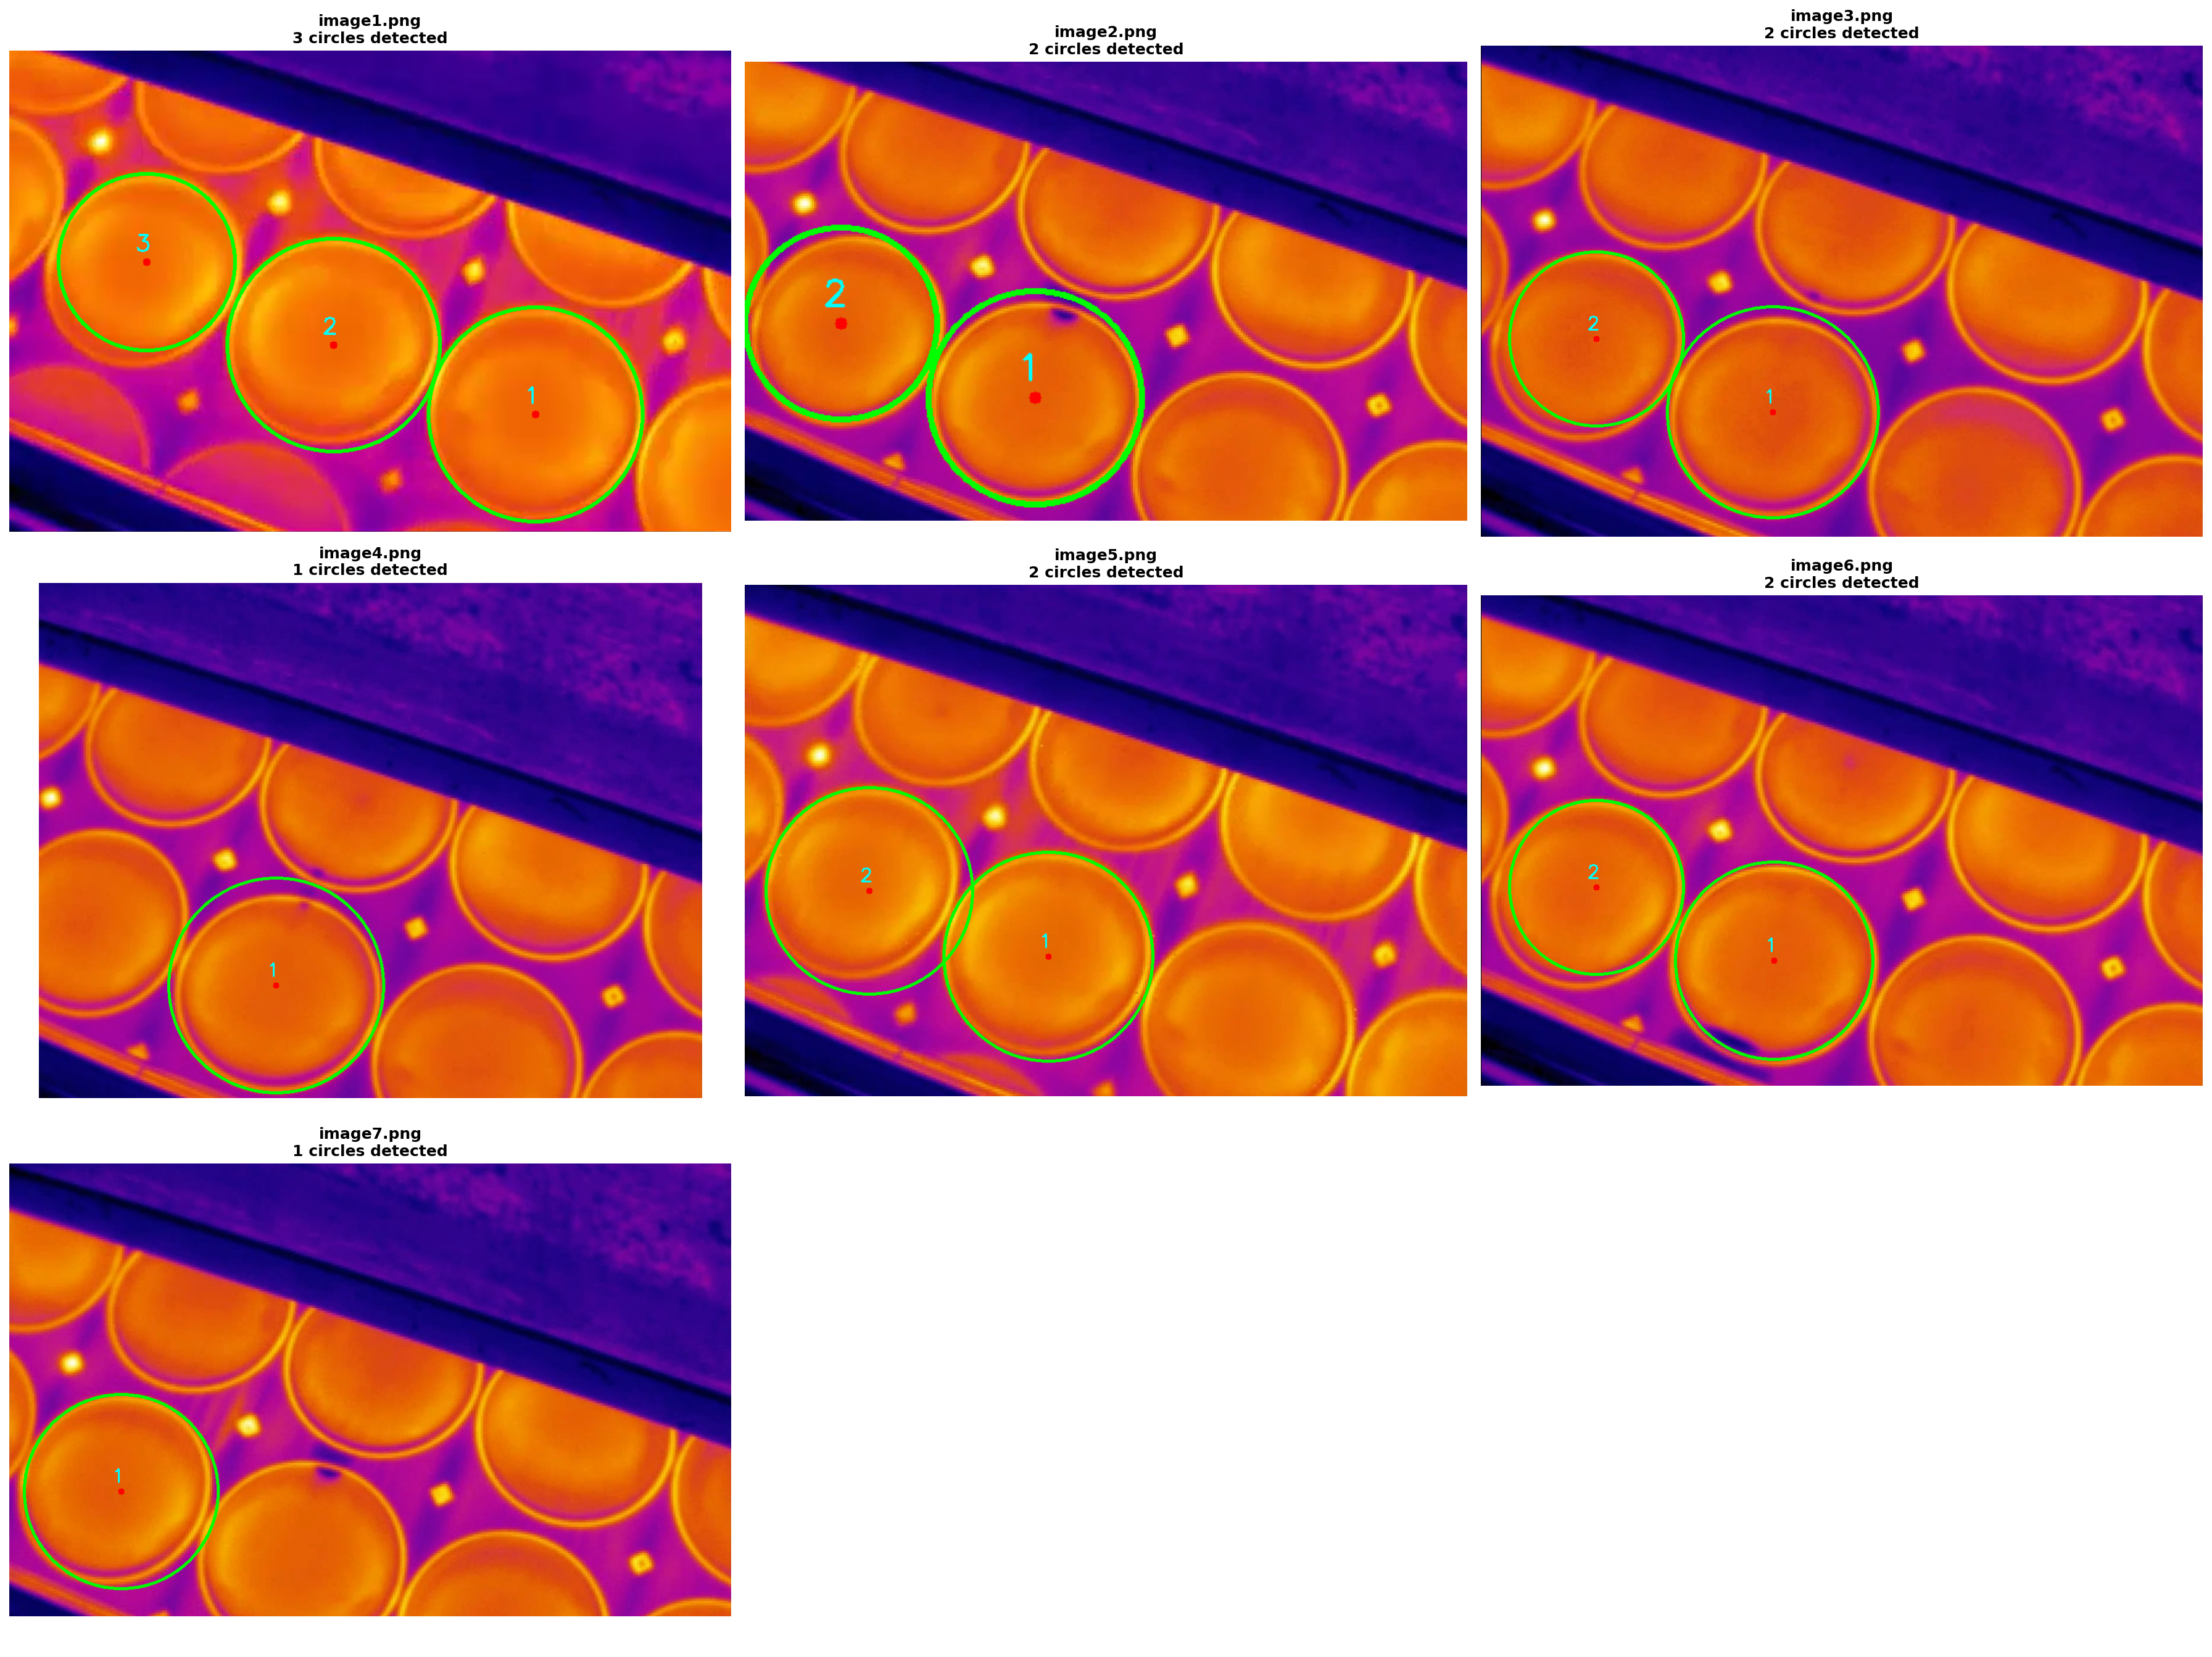
\includegraphics[width=0.9\textwidth]{Results/visualizations/all_results.png}
\caption{Combined detection results showing all processed images in a grid layout. Each image displays detected circles with green outlines, red center points, and yellow numbered labels.}
\label{fig:all_results}
\end{figure}

\subsubsection{Statistical Analysis}

\begin{figure}[H]
\centering
\includegraphics[width=0.85\textwidth]{Results/visualizations/circle_counts.png}
\caption{Bar chart showing the number of circles detected in each image. Value labels on top of bars indicate exact counts.}
\label{fig:circle_counts}
\end{figure}

\begin{figure}[H]
\centering
\includegraphics[width=0.75\textwidth]{Results/visualizations/radius_distribution.png}
\caption{Histogram of radius distribution across all detected circles. Red dashed line indicates mean radius, green dashed line shows median.}
\label{fig:radius_dist}
\end{figure}

\begin{figure}[H]
\centering
\includegraphics[width=0.85\textwidth]{Results/visualizations/radius_boxplot.png}
\caption{Box plot showing radius distribution by image. Boxes indicate quartiles, whiskers show range, and outliers are plotted individually.}
\label{fig:radius_boxplot}
\end{figure}

\begin{figure}[H]
\centering
\includegraphics[width=0.7\textwidth]{Results/visualizations/summary_table.png}
\caption{Summary statistics table with key metrics including total images processed, circles detected, and radius statistics.}
\label{fig:summary_table}
\end{figure}

\subsubsection{Debug Visualizations}

\begin{figure}[H]
\centering
\includegraphics[width=0.9\textwidth]{Results/masks/roi_masks_image1.png}
\caption{ROI detection masks for image1.png showing: (a) HSV color mask, (b) Otsu threshold mask, (c) Percentile mask, (d) Adaptive threshold mask, (e) Final combined ROI mask, (f) Original image. This multi-method approach ensures robust ROI detection.}
\label{fig:roi_masks}
\end{figure}

\subsection{Performance Analysis}

\subsubsection{Computational Complexity}
The preprocessing step has complexity $O(wh)$ where $w \times h$ represents the image size. ROI detection requires $O(wh)$ operations for each method applied. The Hough Transform exhibits complexity $O(wh \cdot N_r \cdot N_\theta)$ where $N_r$ denotes the radius range and $N_\theta$ represents the angular resolution. Finally, quality assessment operates with complexity $O(n \cdot N_s)$ where $n$ is the number of detected circles and $N_s = 36$ represents the number of perimeter samples.

\subsubsection{Processing Time}
Average processing time per image: 2-5 seconds (depending on image size and complexity).

\subsection{Quality Metrics}

The strict filtering criteria ensure high precision by detecting only complete, high-quality circles. The edge quality threshold eliminates spurious detections, resulting in a low false positive rate. Furthermore, the multi-method ROI detection approach provides robustness when handling varying thermal patterns across different imaging conditions.

\section{Technical Implementation}

\subsection{Software Stack}
The system is implemented in Python 3.8 or higher. Core libraries include OpenCV 4.5+ for computer vision operations, NumPy 1.19+ for numerical computations, and Matplotlib 3.3+ for visualizations.

\subsection{Code Organization}
\begin{verbatim}
Assignment 1/
|--- main.py                    # Entry point, batch processing
|--- circle_detector.py         # Core detection logic
|--- visualization.py           # Visualization and reporting
|--- config.py                  # Centralized configuration
|--- requirements.txt           # Python dependencies
`-- Results/                   # Output directory
    |--- visualizations/        # 5 separate chart files
    |--- detection_report.json  # Machine-readable results
    |--- detection_report.txt   # Human-readable report
    |--- images/                # Individual detection results
    |--- masks/                 # ROI visualizations
    |--- intermediate/          # Raw detections
    `-- rejected_circles/      # Filtered circles with reasons
\end{verbatim}

\subsection{Key Features}
The system exhibits several key features that contribute to its effectiveness. The modular architecture ensures separation of concerns for maintainability. Centralized configuration provides a single source of truth for all parameters. Comprehensive logging captures debug information for rejected circles, facilitating troubleshooting. Multiple output formats including JSON, text, and visual reports accommodate different use cases. Finally, separate visualizations deliver clear, non-overlapping statistical charts for enhanced readability.

\section{Discussion}

\subsection{Strengths}
The system demonstrates several key strengths. The multi-method ROI detection approach combines HSV, Otsu, and percentile thresholding to provide robustness across varying thermal patterns. Quality-based filtering effectively eliminates false positives while maintaining true detections through edge quality assessment. Comprehensive reporting with multiple visualization formats aids in result interpretation and system debugging. The modular design facilitates maintenance, extension, and adaptation to new requirements. Finally, centralized parameter configuration allows easy tuning without code modification.

\subsection{Limitations}
Several limitations should be acknowledged. The system operates under a circular shape assumption, detecting only circular patterns while ellipses or irregular shapes remain unhandled. Although configurable, the parameter set may require significant adjustment across different thermal imaging systems to achieve optimal results. The Hough Transform imposes computational costs, particularly for large images or wide radius ranges. Additionally, the intentional rejection of partially occluded circles may prove too strict for certain applications requiring detection under occlusion.

\subsection{Future Improvements}
Several avenues for future enhancement exist. Implementing adaptive parameter selection based on image characteristics would reduce manual tuning requirements. Extending the system to detect elliptical patterns through Hough Ellipse Transform would broaden applicability. Deep learning integration could complement traditional methods with CNN-based circle detection. Optimization for real-time video stream processing would enable dynamic applications. A pyramid-based approach for multi-scale detection would handle varying circle sizes more effectively. Finally, developing methods to estimate complete circles from partial arcs would improve detection under occlusion conditions.

\section{Conclusion}

This work presents a comprehensive automatic circle detection system for thermal images. The system successfully combines classical computer vision techniques with modern software engineering practices to achieve robust, accurate detection.

The balance between detection sensitivity and precision is achieved through configurable parameters, allowing adaptation to specific use cases. The comprehensive reporting and debug visualizations facilitate system tuning and result validation. The modular design ensures the system can be easily extended or integrated into larger computer vision pipelines.


\appendix

\section{Configuration Parameters Reference}

\begin{table}[H]
\centering
\caption{Complete Parameter Reference}
\label{tab:params}
\begin{tabular}{@{}lll@{}}
\toprule
\textbf{Parameter} & \textbf{Default} & \textbf{Description} \\
\midrule
\multicolumn{3}{l}{\textbf{Detection Parameters}} \\
min\_radius & 50 & Minimum circle radius (pixels) \\
max\_radius & 200 & Maximum circle radius (pixels) \\
quality\_threshold & 0.1 & Minimum quality score (0-1) \\
dp & 1 & Accumulator resolution ratio \\
minDist & 90 & Min distance between centers (pixels) \\
param1 & 100 & Canny high threshold \\
param2 & 40 & Accumulator threshold \\
margin & -10 & Edge margin (pixels) \\
roi\_coverage & 0.95 & Min ROI coverage ratio \\
edge\_samples & 36 & Perimeter sample points \\
\midrule
\multicolumn{3}{l}{\textbf{Preprocessing Parameters}} \\
gaussian\_kernel & (15, 15) & Gaussian blur kernel size \\
gaussian\_sigma & 3 & Gaussian blur sigma \\
clahe\_clip\_limit & 2.0 & CLAHE contrast limit \\
clahe\_tile\_size & (8, 8) & CLAHE tile grid size \\
\midrule
\multicolumn{3}{l}{\textbf{ROI Parameters}} \\
intensity\_percentile & 70 & Percentile threshold \\
morph\_kernel\_size & (7, 7) & Morphological kernel size \\
fill\_kernel\_size & (15, 15) & Hole filling kernel size \\
\bottomrule
\end{tabular}
\end{table}

\section{Usage Examples}

\subsection{Basic Usage}
\begin{lstlisting}[caption={Processing All Images}]
# Command line
python main.py

# Python script
from main import process_all_images
process_all_images()
\end{lstlisting}

\subsection{Custom Parameters}
\begin{lstlisting}[caption={Custom Detection Parameters}]
from circle_detector import ImprovedCircleDetector

detector = ImprovedCircleDetector('Images/image1.png')
circles = detector.detect_complete_circles(
    min_radius=30,
    max_radius=150,
    quality_threshold=0.05
)
\end{lstlisting}

\subsection{Configuration Modification}
\begin{lstlisting}[caption={Modifying Global Configuration}]
# Edit config.py
DETECTION_PARAMS['min_radius'] = 30
DETECTION_PARAMS['quality_threshold'] = 0.05

# Then run
python main.py
\end{lstlisting}

\end{document}

